
\chapter{Teorie grafu, logika, matematické struktury}
Reprezentace grafů, podgrafy, stupeň uzlu, cesty a cykly, souvislost grafů, izomorfizmus grafů\\
\section{Grafy}
Alenka ... Naleznete-li zde chybu, tak máte mé svolení opravit ji :D
\subsection{Reprezentace grafů}

\textbf{Reprezentace grafů}:
\begin{itemize}
    \item Obrázkem,
    \item Kroužky na klíče a provázkem
    \item Maticí sousednosti: Čtvercová matice zachycující, které vrcholy spolu sousedí. Sousedí = 1, nesousedí = 0. Pro neorientované grafy je matice symetrická, pro orientované nesymetrická,
    \item Maticí incidence: Matice reprezentující vztah mezi vrcholy a hranami. Řádky jsou vrcholy, sloupce hrany. Je-li vrchol incidentní s hranou píšeme 1, v opačném případě 0.
    \item Maticí vzdálenosti: Stejně jako matice sousednosti, jen místo jedniček obsahuje vzdálenosti mezi uzly (délky hran, váhu oblouků),
    \item Laplaceovou maticí,
    \item Seznamem sousedů.
\end{itemize}
%% -----------------------------------------------------------------------------------------------------------------------------

\subsection{Prostý graf, graf, podgraf}

\begin{definition}
\textbf{Prostý (jednoduchý) graf} $G$ se skládá z konečné množiny \textbf{vrcholů (uzlů, nodes)} $n(G)$ a z konečné množiny \textbf{hran (vertices, edges)} $e(G)  \subseteq \{ \{ u, v \} | u,v \in n(G), u \neq v \}$. Řekneme, že hrana $e = \{ u, v \}$ je incidentní s vrcholy $u,v \in n(G)$ nebo že spojuje vrcholy $u,v$.
\end{definition}

\begin{definition}
\textbf{Graf} nebo také \textbf{multigraf} je trojice $G = (n(G), e(G), \varepsilon_G)$, je definován konečnou množinou uzlů $n(G)$, konečnou množinou hran $e(G)$ a zobrazením $\varepsilon_G : e(G) \rightarrow  { n(G) \choose 2 }  \cup n(G)$, kde ${ n(G) \choose 2 }$ označuje množinu všech neuspořádaných párů vrcholů. Hrany, které se zobrazí na $n(G)$ se nazývají \textbf{smyčky}. Graf tedy může mít vrcholy spojené několika hranami a hrany spojující pouze jeden vrchol.
\end{definition}

\begin{definition}
Mějme graf $G$. Graf $G'$ se nazývá \textbf{podgraf} grafu $G$, jestliže $n(G') \subseteq n(G)$, $e(G') \subseteq e(G)$ a zobrazení $\varepsilon_{G'}$ je restrikcí zobrazení $\varepsilon_G$. Pokud $\{ u, v \} \in n(G')$ jsou spojeny hranou v $G$ implikuje, že $\{ u, v \}$ je spojené hranou v $G'$, pak $G'$ je podgraf $G$ \textbf{indukovaný} jeho vrcholy.
\end{definition}
%% -----------------------------------------------------------------------------------------------------------------------------

\subsection{Sled, tah, cesta, kružnice}

\begin{definition}
V grafu $G$ definujeme \textbf{sled (walk)} mezi vrcholy $u,v$ jako alternující posloupnost vrcholů a hran $(u = u_0, e_1, u_1, e_2, \ldots, u_{n-1}, e_n, u_n = v), n > 0$ takovou, že $\varepsilon_G (e_i) = {u_{i-1}, u_i}, 1 \leq i \leq n$. Číslo $n$ pak nazveme \textbf{délkou} sledu.
\end{definition}

\begin{definition}
\textbf{Tah (stopa, cesta, trail)} v grafu $G$ je sled, kde $i\neq j \Rightarrow e_i \neq e_j, 1 \leq , j \leq n $. Neopakují se hrany.
\end{definition}

\begin{definition}
\textbf{Cesta (jednoduchá cesta, path)} v grafu $G$ je sled, kde $i \neq j \Rightarrow u_i \neq u_j, 1 \leq , j \leq n $. Neopakují se vrcholy.
\end{definition}

V celém textu jsou použity pojmy tah a cesta. (Ne cesta a jednoduchá cesta).

\begin{definition}
\textbf{Kružnice (circle)} délky $n$ v grafu $G$ je cesta $(u_0, e_1, u_1, e_2, \ldots, u_{n-1}, e_n, u_n)$, ve které $u_0 = u_n$.
\end{definition}
%% -----------------------------------------------------------------------------------------------------------------------------

\subsection{Souvislý graf, kompletní graf, komponenta grafu, most, stupeň uzlu}

\begin{definition}
Řekneme, že graf je \textbf{souvislý (propojený, connected)}, jestliže zde existuje cesta mezi libovolnými dvěma uzly $u,v$. V opačném případě je graf \textbf{nesouvislý}.
\end{definition}

\begin{definition}
Graf je \textbf{kompletní (úplný, complete)}, jestliže mezi každými dvěma vrcholy existuje hrana. 
\end{definition}

\begin{definition}
Graf $K$ je \textbf{komponentou (částí)} grafu $G$, jestliže $K$ je maximální souvislý podgraf grafu $G$.
\end{definition}

\begin{theorem}
Graf je souvislý právě tehdy, když má jen jednu komponentu.
\end{theorem}

\begin{definition}
Řekneme, že hrana $e$ v grafu $G$ je \textbf{most}, jestliže se po odstranění hrany $e$ zvýší počet komponentů grafu $G$.
\end{definition}

\begin{definition}
\textbf{Stupeň} uzlu $u$ v grafu $G$: $deg(u) = | \{e \in e(G) | \varepsilon_G (e) = \{ u, v \} |$.
\end{definition}

\begin{theorem}
Nechť $G$ je graf a $|e(G)| = m$. Potom
$$ \sum_{u \in n(G)} deg(u) = 2m.$$
\end{theorem}
%% -----------------------------------------------------------------------------------------------------------------------------

\subsection{Orientovaný graf, indegree, outdegree, další orientované pojmy}

\begin{definition}
\textbf{Orientovaný graf (directed graph, digraph)} $D$ se skládá z konečné množiny vrcholů $n(D)$, konečné množiny \textbf{oblouků (arcs)} $a(D)$ a zobrazení $\varepsilon_D : A \rightarrow \{ (u, v) | u,v \in n(D) \}$, které přiřazuje uspořádanou dvojici uzlů $(u,v)$ každému oblouku $a \in a(D)$. Řekneme, že oblouk $a$ jde z uzlu $u$ do uzlu $v$.
\end{definition}

\begin{definition}
Nechť $D$ je orientovaný graf. Pro uzel $u \in n(D)$ definujeme množiny:
$$ A_{in} = \{ a \in a(D) | \exists v \in n(D) : \varepsilon_D (a) = (v, u) \},$$
$$A_{out} = \{ a \in a(D) | \exists v \in n(D) : \varepsilon_D (a) = (u, v) \}.$$
Pak \textbf{vstupní stupeň (indegree)} uzlu $u$ je definováno jako $deg_+ (u) = |A_{in}|$, a \textbf{výstupní stupeň (outdegree)} uzlu $u$ $deg_- (u) = |A_{out}|$. Tedy indegree je počet oblouků vedoucí do uzlu, outdegree počet oblouků vedoucí z uzlu.
\end{definition}

\begin{definition}
Je-li $deg_- (u) = 0$, nazveme $u$ \textbf{koncovým uzlem}, je-li $deg_+ (u) = 0$, nazveme $u$ \textbf{počátečním uzlem} orientovaného grafu $D$.
\end{definition}

\begin{definition}
Podobně jako u neorientovaných grafů definujeme \textbf{orientovaný sled, orientovaný tah, orientovanou cestu, orientovanou kružnici = cyklus}. Jediným rozdílem je to, že místo hran používáme oblouky.
\end{definition}
%% -----------------------------------------------------------------------------------------------------------------------------

\subsection{Zorientování grafu, symetrizace digrafu, souvislý digraf}

\begin{definition}
Mějme prostý graf $G$. Orientovaný graf $D$ definujeme tak, že pro každou hranu $\{ u, v\} \in e(G)$ jsou v $D$ právě dva oblouky $a, a'$ takové, že $\varepsilon_D (a) = (u, v)$ a $\varepsilon_D (a') = (v,u)$ a $a(D)$ neobsahuje žádné další oblouky. Řekneme, že takový graf $D$ byl vytvořen \textbf{ symetrickým zorientováním} grafu $G$. Tedy každá hrana je nahrazena dvěma oblouky.
\end{definition}

\begin{definition}
Mějme prostý graf $G$. Definujeme orientovaný graf $D$ tak, že pro každou hranu $\{ u, v \} \in e(G)$ je v a(D) jeden oblouk $a$ takový, že $\varepsilon_D (a) = (u, v)$ nebo $\varepsilon_D (a) = (v,u)$ a $a(D)$ neobsahuje žádné další oblouky. Řekneme, že takový graf $D$ byl vytvořen \textbf{zorientováním} grafu $G$. Každá hrana je tedy nahrazena jedním obloukem. Takto vytvořený graf neobsahuje cykly délky dva.
\end{definition}

\begin{definition}
Nechť $D$ je orientovaný graf. Pak zde existuje jediný prostý graf $G$, který je symetrizací digrafu $D$. Položme $a(D) = \{ \{ u, v \} | u, v \in n(G), u \neq v, \exists a \in A : \varepsilon_D (a) = (u,v) \vee \varepsilon (a) = (u, u) \}$. Tedy oblouky i smyčky jsou nahrazeny jednou hranou mezi uzly.
\end{definition}

\begin{definition}
Řekneme, že digraf je \textbf{souvislý}, jestliže je souvislá jeho symetrizace.
\end{definition}

\begin{definition}
Řekneme, že digraf $D$ je \textbf{silně souvislý}, jestliže pro jakékoli dva vrcholy $u, v \in n(D)$ je v $D$ orientovaná cesta z $u$ do $v$. Zřejmě každý silně souvislý graf je souvislý, naopak to platit nemusí.
\end{definition}
%% -----------------------------------------------------------------------------------------------------------------------------

\subsection{Izomorfismus}

\begin{definition}
Dva grafy $G$ a $G'$ nazýváme \textbf{izomorfní}, jestliže existuje bijektivní zobrazení $f: n(G) \rightarrow n(G')'$ tak, že platí:
$\{ x, y \} \in e(G)$, právě když $\{f(x), f(y) \} \in e(G')$. Tedy grafy $G$ a $G'$ se liší pouze očíslování vrcholů. (Existuje bijektivní zobrazení mezi vrcholy, které zachovává hrany.)
\end{definition}

\begin{theorem}
Nutné (nikoliv postačující) podmínky pro dva izomorfní grafy:
\begin{itemize}
    \item Mají stejný počet uzlů.
    \item Mají stejný počet hran.
    \item Jejich stupně uzlů seřazené do neklesající posloupnosti jsou shodné.
    \item Každý uzel grafu má sousedy stejného stupně jako odpovídající uzel v grafu izomorfním.
\end{itemize}
\end{theorem}


\section{Speciální grafy}
Stromy, planární grafy, barevnost grafu, hamiltonovské a eulerovské grafy
%% -----------------------------------------------------------------------------------------------------------------------------

\subsection{Strom, kostra, kořenový strom, binární strom}

\begin{definition}
Souvislý graf neobsahující kružnice nazýváme \textbf{strom (tree)}. Strom může mít maximálně jednu hranu spojující dva vrcholy.
\end{definition}


\begin{theorem}
Několik tvrzení o stromech:
\begin{itemize}
    \item V grafu existuje právě jedna cesta mezi každými dvěma uzly právě tehdy, když je graf strom.
    \item Každá hrana je most právě tehdy, když je graf strom.
    \item Souvislý graf $G$ má $n$ uzlů a $n-1$ hran právě tehdy, když je to strom.
    \item Jakýkoli graf $G$ s $n$ uzly, $n-1$ hranami, který neobsahuje kružnice a je souvislý je strom.
    \item Nechť $T$ je strom. Vytvoříme-li graf $T'$ přidáním nové hrany do grafu $T$, pak graf $T'$ obsahuje právě jednu kružnici.
    \item Jestliže přidání nové hrany do grafu $G$ (který neobsahuje žádnou kružnici) implikuje vznik právě jedné kružnice, pak je graf $G$ strom.
\end{itemize}
\end{theorem}

\begin{definition}
Podgraf $T$ grafu $G$ s $n$ vrcholy nazveme \textbf{kostra (spanning tree)} grafu $G$, jestliže je $T$ strom s $n$ vrcholy.
\end{definition}

\begin{theorem}
Nechť $G$ je prostý graf s $n$ vrcholy. Jestliže podgraf $H$ grafu $G$ má $n$ uzlů a jestliže platí dvě z následujících vlastností, pak platí i třetí vlastnost.
\begin{itemize}
    \item $H$ je souvislý,
    \item $H$ má $n-1$ hran,
    \item $H$ neobsahuje kružnici.
\end{itemize}
\end{theorem}

\begin{theorem}
Ve stromu $T$ s alespoň dvěma vrcholy jsou nejméně dva vrcholy se stupněm uzlu rovno jedné.
\end{theorem}

\begin{theorem}[Cayley]
Nechť $K_n$, $n \geq 2$, je kompletní graf. Pak $K_n$ má $n^{n-2}$ koster.
\end{theorem}

\begin{definition}
Vrchol stromu může být specifikovaný jako jeho kořen. Z nějakého důvodu se takové stromy kreslí s kořenem nahoře. Strom s kořenem nazveme \textbf{kořenový strom (rooted tree)}.
\end{definition}

\begin{definition}
Hrany kořenového stromu jsou často uvažovány jako orientované. Každý nekořenový vrchol má právě jednu hranu vedoucí směrem ke kořenu. \textbf{Potomek (descendant)} uzlu v orientovaném grafu je definován jako jakýkoli uzel dosažitelný z tohoto uzlu. Často se vrcholy blíže ke kořenu označují jako \textbf{rodiče (parents)}, vrcholy dále od kořenu jako \textbf{děti (children)}. Vrcholy, které mají jen jednu hranu (jsou tedy na opačném konci než kořen), se nazývají \textbf{listy (leaves)}.
\end{definition}

\begin{definition}
\textbf{Binární strom (binary tree)} je kořenový strom, ve kterém má každý uzel nejvýše dva potomky. \textbf{Výška (hloubka, depth)} binárního stromu je číslo říkající, kolik uzlů musíme projít od kořene k nejvzdálenějšímu listu.
\end{definition}

\begin{definition}
\textbf{Vyvážený binární strom (balanced binary tree)}: Výška jeho listů se liší nejvýše o jeden. U takového stromu lze předpovědět jeho výšku, ta je rovna celé části $log_2 n$, kde $n$ je počet uzlů binárního vyváženého stromu.
\end{definition}

\begin{definition}
\textbf{Binární vyhledávací strom (binary search tree)}: Binární strom, jehož uzlům jsou přiřazeny klíče z uspořádané množiny. Levý podstrom obsahuje pouze klíče, které jsou menší než klíč uzlu. Pravý podstrom obsahuje klíče které jsou větší než klíč uzlu.
\end{definition}

\begin{definition}
\textbf{Halda (heap)} je vyvážený vyhledávací strom, kde každý potomek má menší (nebo větší) číslo než rodič. Tedy kořen má vždy největší (nejmenší) číslo.
\end{definition}

\subsection{Planární grafy}

\begin{definition}
Graf $G$ je \textbf{planární}, jestliže jeho vrcholy mohou být reprezentovány body v rovině, hrany mohou být reprezentovány spojitou čárou spojující tyto body a žádné dvě hrany se nesmí protínat. Takovou reprezentaci grafu nazveme \textbf{rovinnou reprezentací (plane embedding)}.
\end{definition}

\begin{definition}
Nechť $H$ je rovinná reprezentace grafu $G$. Dvoudimenzionální oblasti obraničené hranami v $e(H)$ se nazývají \textbf{stěny (buňky, faces)}, vrcholy a hrany okolo stěn nazýváme \textbf{hranice (boundaries)}.
\end{definition}


\begin{theorem}[Euler]
Nechť $H$ je rovinná reprezentace souvislého planárního grafu který má $n$ vrcholů, $m$ hran a $f$ stěn. Pak $n - m + f = 2$.
\end{theorem}

\begin{theorem}
Nechť $G$ je prostý souvislý planární graf s $n$ vrcholy a $m$ uzly. Pak $m \leq 3n - 6$.
\end{theorem}

\begin{definition}
Dva grafy $G_1$ a $G_2$ jsou \textbf{homeomorfní (homeomorphic)} (nebo identické do vrcholu stupně 2), pokud je můžeme obdržet z grafu $G_3$ vložením nových vrcholů stupně $2$ do jeho hran. (Existuje zobrazení, které nemusí být bijektivní, mezi vrcholy, které zachovává hrany.)
\end{definition}

\begin{theorem}
Dva grafy $G_1$ a $G_2$ jsou homeomorfní, jestliže jsou izomorfní až na uzly stupně dva.
\end{theorem}

\begin{theorem}
Homeomorfismus zachovává planaritu.
\end{theorem}

\begin{theorem}
Graf je planární právě tehdy, když neobsahuje $K_5$ nebo $K_{3,3}$ jako podgrafy.
\end{theorem}

\begin{theorem}
Každý planární graf je $5$-obarvitelný. A dokonce každý planární graf je i $4$-obarvitelný. (Ne každý. Graf musí mít alespoň 4 uzly, aby byl 4-obarvitelný)
\end{theorem}
%% -----------------------------------------------------------------------------------------------------------------------------

\subsection{Barevnost grafu, chromatické číslo, diskrétní graf, kompletní graf, bipartita}

\begin{definition}
Graf (neorientovaný!) bez smyček je \textbf{obarvitelný}, jestliže každému jeho vrcholu lze přiřadit barvu tak, aby jakékoli dva sousedící vrcholy (vrcholy spojené hranou) měly jinou barvu.
\end{definition}

\begin{definition}
Jesliže je $G$ obarvitelný $k$ barvami řekneme, že je \textbf{$k$-obarvitelný}. Nejmenší takové $k$ se nazývá \textbf{chromatické číslo} grafu $G$ a píšeme $\chi(G) = k$.
\end{definition}

\begin{definition}
Graf $D_n$ nazveme \textbf{diskrétní}, jestliže $|n(D_n)| = n > 0$ a $e(D_n) = \emptyset$. 
\end{definition}

\begin{definition}
prostý graf $K_n$ s $n$ vrcholy, $n >0$, bez smyček takový, že jakékoli dva jeho uzly jsou spojené hranou se nazývá kompletní.
\end{definition}

\begin{definition}
prostý graf $K_{p,q}$ s $n(K_{p,q}) = P \cup Q, |P| = p, |Q| = q$ a $e(K_{p,q})$ obsahující pouze dvojice $(r,s)$ vrcholů takové, že $r \in P, s \in Q$, se nazývá \textbf{bipartita}. Pokud navíc $e(K_{p,q})$ obsahuje všechny dvojice $(r,s)$ takové, že $r \in P, s \in Q$, pak $K_{p,q}$ nazveme \textbf{kompletní bipartitou}.
\end{definition}

\begin{theorem}
Je jednoduché ukázat:
\begin{itemize}
    \item $\chi(G)=1$ právě tedy, když $G=D_n$.
    \item $\chi(K_n)=n$
    \item $\chi(K_{p,q})=2$ jestliže $e(K_{p,q}) \ne \emptyset$
\end{itemize}
\end{theorem}

\begin{theorem}
Kružnice je $2$-obarvitelná právě tehdy, když má sudý počet uzlů. Tedy graf neobsahující žádnou lichou kružnici je $2$-obarvitelný a graf obsahující lichou kružnici není $2$-obarvitelný. Strom je také $2$-obarvitelný.
\end{theorem}
%% -----------------------------------------------------------------------------------------------------------------------------

\subsection{Hamiltonovské a Eulerovské grafy}

\begin{definition}
Graf $G$ nazveme \textbf{Hamiltonovským}, pokud obsahuje kružnici procházející každým uzlem v $G$ právě jednou.
\end{definition}

\begin{theorem}[Ore]
Nechť $G$ je graf s $n$ uzly a nechť $deg(u) + deg(v) \geq n$ pro každé dva uzly $u,v$, které nejsou spojeny hranou v $G$. Pak $G$ je Hamiltonský graf.
\end{theorem}

\begin{theorem}[Dirac]
Nechť $G$ je graf s $n$ uzly a nechť $deg(u) \geq \frac{n}{2}$ pro každý uzel $u \in n(G)$. Pak $G$ je Hamiltonský graf.
\end{theorem}

Obě věty jsou postačujícími podmínkami. Diracova věta je víc nadbytečnější.

\begin{definition}
Graf $G$ je \textbf{Eulerovský}, jestliže existuje v $G$ uzavřený tah obsahující všechny hrany $G$. Graf $G$ je \textbf{semi-Eulerovský}, jestliže existuje v $G$ tah obsahující všechny hrany $G$.
\end{definition}

\begin{theorem}
Nechť $G$ je souvislý graf. Pak $G$ je Eulerovský právě tehdy, když každý jeho uzel má sudý stupeň. Graf $G$ je semi-Eulerovský právě tehdy, když jsou v $G$ právě dva uzly lichého stupně.
\end{theorem}
%% -----------------------------------------------------------------------------------------------------------------------------

\subsection{Turnaj, Hamiltonovské a Eulerovské orientované grafy}

\begin{definition}
Digraf $D$ nazveme \textbf{turnaj (tournament)}, jestliže pro jakékoli dva vrcholy $u, v \in n(D)$ existuje jeden oblouk $a \in a(D)$ takový, že platí $\varepsilon_D (a) = (u,v)$ nebo $\varepsilon_D (a) = (v,u)$. Tedy ke každému páru různých vrcholů zde existuje pouze jeden oblouk, který je spojuje.
\end{definition}

\begin{theorem}
Nechť $T$ je turnaj a $v$ je jeho vrchol s maximálním outdegree. Pak pro každý uzel $w \in n(D)$, $w \neq v$, existuje orientovaná cesta z $v$ do $w$ přes nejvýše dva oblouky. (Buď ho porazil a nebo porazil někoho, kdo ho porazil.)
\end{theorem}

\begin{theorem}
V každém turnaji existuje orientovaná Hamiltonská cesta.
\end{theorem}

\begin{theorem}
Jestliže je $T_n$ silně souvislý turnaj s $n$ vrcholy, $n >2$, pak $T_n$ obsahuje cykly délky $3,4, \ldots, n$.
\end{theorem}

\begin{theorem}
Turnaj $T_n$ je Hamiltonský právě tehdy, když je silně souvislý.
\end{theorem}

\begin{definition}
Orientovaný graf $D$ nazveme \textbf{Eulerovským}, jestliže v $D$ existuje uzavřený orientovaný tah procházející všechny jeho oblouky.
\end{definition}

\begin{theorem}
Souvislý digraf $D$ je Eulerovský právě tehdy, když $deg_- (u) = deg_+(u)$ pro každý vrchol $u \in n(D)$.
\end{theorem}

\section{Optimalizační úlohy na grafech}
Algoritmy pro úlohy řešitelné v polynomiálním čase (minimální kostra grafu, nejkratší cesty v grafu, maximální tok v síti)
\subsection{Vážený graf, minimální kostra grafu, Kruskal, Prim}

\begin{definition}
Nechť $G$ je prostý graf. Jestliže je dáno zobrazení $w: e(G) \rightarrow \mathbb{R}$, pak řekneme, že graf $G$ je \textbf{vážený (weighted)}. Reálná čísla přiřazená každé hraně nazveme \textbf{váhy (ceny, délky, weight, price, length)}. Jestliže $G'$ je podgraf grafu $G$, pak váhu (délku, cenu) grafu $G'$ definujeme jako $w(G') = \sum_{e \in e(G')} w(e)$.
\end{definition}

\begin{definition}
Nechť $S$ je kostra jednoduchého grafu $G$. Řekneme, že $S$ je minimální kostra grafu $G$, jestliže $w(S) \leq w(T)$ pro každou kostru $T$ grafu $G$.
\end{definition}

\begin{theorem}
Nechť $G$ je prostý vážený graf s váhami $W$ a nechť $C = (v_0, e_1, v_1, e_2, v_2, \ldots, v_{p-1}, e_p, v_p = v_0$ je kružnice v $G$. Jestliže $w(e_1) > w(e_i)$ pro $2\leq i \leq p$, kde hrana $e_1$ nemůže být obsažena v žádné minimální kostře $G$.
\end{theorem}

\begin{theorem}
Nechť $G$ je prostý vážený graf s váhami $W$ a nechť $(v_0, e_1, v_1, e_2, v_2, \ldots, v_{p-1}, e_p, v_p = v_0$ je kružnice v $G$. Pokud $w(e_1) > w(e_i)$ pro $2\leq i \leq p$, pak je zde alespoň jedna minimální kostra v $G$ která neobsahuje $e_1$.
\end{theorem}
\textbf{Kruskalův-Borůvkův algoritmus}\\
Nechť $G$ je vážený prostý souvislý graf s $n$ uzly a $k$ hranami. Označme $A = [e_1, e_2, \ldots, e_k ]$ matici hran v $G$, ve které jsou váhy v rostoucím pořadí. Indexování začínáme od 0. Pro matici $A$ délky $k$, $m<k$, definujme $A[m:] := [A[m], A[m+1], \ldots, A[k+1]]$. Krok po kroku pak vytváříme grafy $S_1, S_2, \ldots, S_m$, kde $S_m$ je hledaná minimální kostra grafu. Každý z grafů má stejnou množinu vrcholů $n(G)$ a množinu hran následující:
\begin{enumerate}
    \item $e(S_1) := [A[0]], A = A[1:]$,
    \item Jestliže $S_i$ je souvislá a je to kostra a algoritmus končí. Jinak pokračujte na krok $3$.
    \item Jestliže přidání hrany $A[0]$ do $S_i$ vytvoří kružnici, pak $A := A[1:]$, jinak položme $e(S_{i+1}) := e(S_i) \cup \{ A[0] \}, A:= A[1:]$. A jdi na krok 2.
\end{enumerate}

Tedy Kruskalův algorismus vytváří kostru krok po kroku přidáváním hran z posloupnosti hran, které jsou uspořádány v rostoucím pořadí dle jejich vah. Jestliže přidáním hrany má vzniknout kružnice, pak tuto hranu vyřadíme.
\\

\textbf{Primův-Jarníkův algoritmus}\\
Nechť $G$ je vážený prostý souvislý graf s $n$ uzly. Pro podgraf $S$ grafu $G$, který neobsahuje kružnici, označme $S^+$ graf vytvořený přidáním vrcholu $v$ a hrany $e$ do $S$ tak, že $e$ je hrana s poslední váhou $w(e)$ spojující vrchol $v$ s jiným vrcholem ve $V$. V následujících krocích jsou grafy $S_1, S_2, \ldots, $ utvořeny následovně.
\begin{enumerate}
    \item $n(S_1)=\{u,v\},e(S_1)=\{e=\{u,v\}\})$ s $e=\{u,v\}$ mající poslední váhu,
    \item Jestliže $|e(S_i)|=n-1$, $S_i$ je minimální kostra, algoritmus skončí,
    \item jinak klademe $S_{i+1}:=S^{+}_{i}$, jdi na 2.
\end{enumerate}

\subsection{Délka orientované cesty, nejkratší cesta, Dijkstra, Warshall-Floyd}

V následujícím textu bude grafem vždy myšlen prostý orientovaný graf $G$. 

\begin{definition}
Každému obloku $c \in a(G)$ přiřadíme reálné číslo $l(c)$, které nazýváme \textbf{délka} $c$. \textbf{Délka orientované cesty} $p$ v $G$ je definována jako suma délek všech oblouků v $p$ a značíme ji $l(p)$.
\end{definition}

\begin{definition}
Pro dva vrcholy $u,v \in n(G)$ uvažujme množinu $P(u,v)$ všech orientovaných  cest z $u$ do $v$. Položme $d(u,v) = \min_{p \in P(u,v)} \{ l(p)\}$. Pokud je $d(u,v)$ konečné číslo, pak je nezveme \textbf{vzdáleností (distance)} z $u$ do $v$. Cesta, pro kterou platí $l(p) = d(u,v)$, se nazývá \textbf{minimální cesta (minimal path)} z $u$ do $v$. Pokud žádná taková cesta neexistuje, tak píšeme $d(u,v) = \infty$, a pokud minimum neexistuje, píšeme $d(u,v) = -\infty$.
\end{definition}

Délka oblouků může být i záporná, ale hledání minimální cesty v grafu s cyklem záporné délky nedává smysl. Některé algoritmy proto pracují jen s kladnými cestami (Dijkstra).

Definice problému: Nechť $G$ je prostý orientovaný graf, k jehož obloukům jsou přiřazeny jen kladné délky a nechť $s \in n(G)$. Pro každé $v \in n(G)$ najděte vzdálenost, minimální cestu $p(s,v)$ a její délku.

Horní odhad vzdálenosti $d(s,v)$ je nějaké číslo $D(v)$ takové, že $D(v) \geq d(s,v)$. 

Pro každé $v \in n(G)$ označíme $\pi(v)$ vrchol bezprostředně předcházející $v$ v minimální cestě z $s$ do $v$ konstruované Dijkstrovým algoritmem. Pokud taková cesta ještě nebyla konstruována, klademe $\pi(v) = \emptyset$.

Pro každé $u \in n(G)$ označuje $N(u) = \{ v \in n(G) | (u,v) \in a(G) \}$ množinu všech vrcholů do nichž vede oblouk z $u$.

Symbol $S$ označuje množinu všech vrcholů, pro které Dijkstrův algoritmus už našel minimální cestu. Klademe $Q = n(G) - S$.

\textbf{Dijkstrův algoritmus}
\begin{enumerate}
    \item Inicializace: Pro každé $u\in n(G)$, klademe $\pi(u)=\emptyset$, $D(s)=0$, $D(u)=\infty$ pro $u\neq s$, $S=\emptyset$, $Q=n(G)$.
    \item Test pro ukončení: Jestliže $S=n(G)$, jdi na 5.
    \item Určení pevného uzlu: V $Q$, najdi vrchol $v$ s posledním $D(v)$ a přidej ho k $S$. Jestliže $D(u)=\infty$ pro všechna $u\in Q$, jdi na 5.
    \item Zlepšení horního odhadu: Položme $D(w)=D(v)+l((v,w))$ a
$\Pi(w)=v$ pro každé $w \in \mathcal{N} (v)  \cap Q$ tak, že $D(w)> D(v)+l((v,w))$. Jdi na 2.
    \item Generování minimální cesty: Žádná cesta neexistuje z $s$ do vrcholů zbývajích v $Q$. Pro všechny další vrcholy položme $d(s,v)=D(v)$ a generujeme cestu $p$ z $s$ do $v$ otočením cesty 
$v\rightarrow\pi(v)\rightarrow\pi(\pi(v))\rightarrow\pi(\pi(\pi(v)))\rightarrow\cdots\rightarrow s$.
\end{enumerate}


\textbf{Warshall-Floydův algoritmus}\\
Dijkstrův algoritmus nefunguje pro grafy obsahující cykly záporných délek. Pro takové grafy lze použít Warshall-Floydův algoritmus. Máme-li dané délky oblouků, pak tento algoritmus najde minimální cestu mezi jakýmikoli dvěma uzly. Pokud taková cesta neexistuje (z důvodu záporného cyklu), tento algoritmus ji zdetekuje. Tj. na diagonále matice $A$ se objeví záporné číslo.

Uvažujme prostý orientovaný graf $G$ s $n$ vrcholy. Algoritmus pracuje se dvěma $n \times n$
maticemi $A$ a $P$. Do matice $A$ na pozici $a_{i,j}$ zapíšeme délky oblouku vedoucího z vrcholu $i$ do vrcholu $j$. V matici $P$ položíme prvek $p_{i,j} = j$.

Algoritmus má vždy $n$ kroků. Začínáme s maticemi $A_0$, $P_0$. V $i$-tém kroku jsou matice $A_i$, $P_i$ vytvořeny z matic $A_{i-1}$, $P_{i-1}$. Po $n$ krocích obdržíme matice $A_n$, $P_n$, které mají následující význam: V prvku $a_{i,j}$ je délka minimální cesty z vrcholu $i$ do vrcholu $j$. Je-li $p_{i,j} = k$, pak $(i,k)$ je první oblouk minimální cesty z $i$ do $j$.

Známe-li prvky $a^{i-1}_{i,j}$ a $p^{i-1}_{i,j}$ matic $A^{i-1}$ a $P^{i-1}$,
můžeme spočíst prvky $a^{i}_{i,j}$ a $p^{i}_{i,j}$ matic $A^{i}$ a $P^{i}$ následovně: Pokud $a^{k-1}_{i,k}+a^{k-1}_{k,j} \leq a^{k-1}_{i,j}$, pak $a^k_{i,j}=a^{k-1}_{i,k}+a^{k-1}_{k,j}$,  $p^k_{i,j}=k$. Jinak $a^k_{i,j}=a^{k-1}_{i,j}$,  $p^k_{i,j}=p^{k-1}_{i,j}$.

\subsection{Maximální tok v síti, Ford-Fulkerson}

\begin{definition}
\textbf{Síť (network)} je čtveřice $N = (G, s, t, c)$, kde $g$ je prostý orientovaný graf. Každé uspořádané dvojici vrcholů $(u,v)$ je přiřazena nenegativní \textbf{kapacita} $c(u,v)$. A pro každou dvojici $(u,v) \notin a(G)$ přiřadíme $c(u,v) = 0$. Písmena $s$ a $t$ značí \textbf{zdroj (source)} a \textbf{cíl (target)}.
\end{definition}

V následujícím předpokládáme, že každý vrchol leží na orientované cestě ze zdroje do cíle.

\begin{definition}
\textbf{Tok (flow)} v síti $N=(G,s,t,c)$ je zobrazení $f:n(G) \times n(G) \rightarrow \mathbb{R}$, které splňuje následující tři podmínky:
\begin{enumerate}
    \item $f(u,v) \leq c(u,v), \forall u, v, \in n(G),$
    \item $f(u,v) = -f(u,v), \forall u,v \in n(G),$
    \item $\sum_{v \in n(G)} f(u,v) = 0, \forall u \in n(G) - {s,t}.$
\end{enumerate}
Hodnota, která může být pozitivní, nulová nebo negativní, se nazývá \textbf{tok z uzlu $u$ do uzlu $v$}. Hodnota $|f| = \sum_{v \in n(G)} f(s,u)$ se nazývá \textbf{totální tok (total flow)} sítě $N$.
\end{definition}

Pár poznámek:
\begin{itemize}
    \item Z podmínky $2$ plyne, že $f(u,u) = 0, \forall u \in n(G)$. Tedy tok z uzlu do toho samého uzlu je nula.
    \item Z podmínky $3$: totální tok z každého uzlu (různého od zdroje a cíle) je roven jedné. Dle podmínky $2$ lze zapsat: $\sum_{v \in n(G)} f(u,v) = 0 \forall v \in V - {s,t}$, tedy totální tok do každého uzlu (různého od zdroje a cíle) je nula.
    \item Jestliže neexistuje oblouk mezi uzly $u$ a $v$, nemůže zde být ani tok, protože $c(u,v) = c(v,u) = 0$ a tak $f(u,v) \leq 0$ a $f(v,u) \leq 0$. Z podmínky $2$ pak máme: $f(u,v) = f(v,u) = 0$.
\end{itemize}

V dalším použijeme označení: $f(X,Y)=\sum\limits_{x\in X}\sum\limits_{y\in Y}f(x,y)$ a $n(G) - s$ bude označení pro $n(G) - \{ s \}$.

\begin{theorem}
Nechť $N = (G,s,t,c)$ je síť, kde $G$ je prostý orientovaný graf. Nechť $X, Y, Z \subseteq n(G)$ a nechť $f$ je tok v $N$. Pak
\begin{itemize}
    \item $f(X,X)=0$,
    \item $f(X,Y)=-f(Y,X)$,
    \item jestliže $X\cap Y=\emptyset$, pak $f(X\cup Y,Z)=f(X,Z)+f(Y,Z)$
a $f(Z,X\cup Y)=f(Z,X)+f(Z,Y)$
\end{itemize}
\end{theorem}

\begin{definition}
Nechť $f$ je tok v síti $N = (G, s, t, c)$, kde $G$ je prostý orientovaný graf. Pro každou uspořádanou dvojici vrcholů $(u,v), u,v \in n(G)$ definujeme \textbf{zbytkovou kapacitu (residual capacity)} jako $c_f (u,v) = c(u,v) - f(u,v)$.
\end{definition}
\begin{definition}
Nechť $N = (G, s, t, c)$ je síť a $G$ je prostý orientovaný graf. Nechť $f$ je tok v $N$ a pro každé $u, v \in n(G)$ nechť $c_f (u,v)$ je reziduální kapacita $(u,v)$ v $N$ definována $f$. Pak definujeme prostý orientovaný graf $G_f$, kde $a(G_f) = \{ (u,v) | c_f (u,v) > 0, u,v \in n(G)\}$. Síť $S_f = (G_f, s, t, c_f)$ se nazývá \textbf{zbytkovou síť (residual network)} sítě $N$ vzhledem k toku $f$.
\end{definition}

\begin{theorem}[2]
Nechť $N = (G,s,t,c)$ je síť a $f$ je tok v $N$. Nechť $S_f = (G_f, s, t, c_f)$ je zbytková síť v $N$ vzhledem k $f$ a nechť $f^*$ je tok v $S_f$. Pak zobrazení $(f+f^*) : n(G) \times n(G) \rightarrow \mathbb{R}$ definované jako $(f+f^*) (u,v) = f(u,v) + f^*(u,v)$ je tok v síti $N$.
\end{theorem}

\begin{definition}
Nechť $N = (G, s, t, c)$ je síť. Definujme tok $f$ v $N$ a zbytkovou kapacitu $c_f$ vzhledem k tomuto toku. Nechť $G_f$ je orientovaný graf zbytkové sítě $S_f$ vzhledem k $f$. Nechť $p$ je cesta v $G_f$ ze zdroje $s$ k cíli $t$. Taková cesta se nazývá \textbf{vylepšující cesta (augmenting path)} v $N$ vzhledem k $f$. Nechť $p '(s = u_0, u1, u2, \ldots, u_{k-1}, u_k = t)$. je vylepšující cesta v $n$ vzhledem k $f$. Definujme \textbf{zbytkovou kapacitu (residual capacity)} $c_f (p)$ z $p$ vzhledem k $f$ jako $c_f (p) = \min \{ c_f (u_i, u_{i+1} | 0 \leq i  < k\}$.
\end{definition}

\begin{theorem}[3]
Nechť $N=(G,s,t,c)$ je síť, definujme tok $f$  v $\mathcal{N}$ a zbytkovou síť $S_f=(G_f,s,t,c)$. Nechť
$p=(s=u_0,u_1,u_2,\ldots,u_{k-1},u_k=t)$ je vylepšující cesta v $S_f$ a $c_f(p)$ její zbytková kapacita vzhledem k $f$. Definujme zobrazení $f_p: n(G)\times n(G)\mapsto \mathbb{R}$ následovně:
\begin{itemize}
    \item $f_p(u_i,u_{i+1})=c_f(p),0 \leq i < k$,
    \item $f_p(u_{i+1},u_i)=-c_f(p),0 \leq i < k$,
    \item $f_p(u,v)=0$ jinak.
\end{itemize}
Pak $f_p$ je tok v $G_f$ s $|f_p|=c_f(p) > 0$.
\end{theorem}

\begin{theorem}
Nechť $N=(G,s,t,c)$ je síť, $f$ je tok definovaný v $N$, $S_f=(G_f,s,t,c)$ je zbytková síť vzhledem k $f$ a $p$ je vylepšující cesta v $G_f$ s $c_f (p)$ jako jeho zbytková kapacita. Nechť zobrazení $f_p : n(G) \times n(G) \rightarrow \mathbb{R}$ je definováno stejně jako ve větě 3. Definujme zobrazení $f^{*} = f + f_p : N \times N \rightarrow \mathbb{R}$ jako ve větě 2. Pak $f^{*}$ je tok v $N$ s $ | f^{*} | = |f| + |f_p | > | f |$.
\end{theorem}

\begin{definition}
    Nechť $N=(G,s,t,c)$ je síť, kde $G$ je jednoduchý orientovaný graf. Nechť $(S,T)$ je rozklad $n(G)$ takový, že $s \in S$ a $t \in T$. Pak $(S,T)$ nazveme \textbf{řez (cut)} sítě $N$. Pro rozklad $(S,T)$ tedy máme $S \cup T = n(G)$ a $S \cap T = \emptyset$. Nechť $f$ je tok v $N$, pak lze definovat \textbf{tok přes řez (flow over cut)} $(S,T)$ vzhledem k $f$, značíme $f(S,T)$, a také \textbf{kapacitu řezu (capacity of cut)} $(S,T)$, značíme $c(S,T)$.
\end{definition}

\begin{theorem}
Nechť $N=(G,s,t,c)$ je síť, $f$ je tok definovaný v $N$, a nechť $(S,T)$ je řez $N$. Pak tok přes řez $(S,T)$ vzhledem k $f$ je roven hodnotě $f$, tedy $f(S,T) = |f|$.
\end{theorem}

\begin{theorem}
Hodnota toku v síti není větší než kapacita jakéhokoli řezu v této síti.
\end{theorem}

\begin{theorem}
    Nechť $N=(G,s,t,c)$ je síť a $f$ je tok definovaný v $N$, pak jsou následující tvrzení ekvivalentní:
    \begin{itemize}
        \item $f$ je maximální tok v $N$,
        \item zbytková síť $N_f = (G_f, s, t, c)$ neobsahuje žádnou vylepšující cestu,
        \item $|f| = c(S,T)$ pro řez $(S,T)$ sítě $N$.
    \end{itemize}
\end{theorem}

\textbf{Ford-Fulkersonův algoritmus}\\
Nechť $N=(G,s,t,c)$ je síť, kde $G$ je jednoduchý orientovaný graf.
\begin{enumerate}
    \item Inicializace: Pro každé $u, v \in n(G)$, klademe $f(u,v) = 0$.
    \item Zbytková síť: Pro každé $u, v \in n(G)$ spočteme zbytkovou síť $c_f(u,v) = c(u,v) - f(u,v)$ a získáme zbytkový graf $G_f$ s $a(G_f) = \{ (u,v) | u,v \in n(G), c_f(u,v) > 0 \}$.    
    \item Hledání vylepšující cesty: Neexistuje-li ve zbytkovém grafu $G_f$ žádná vylepšující cesta, algoritmus končí, aktuální celkový tok je maximální. Existuje-li, označíme vylepšující cestu $p = (s = u_0, u_1, \ldots, u_k = t$ a pokračujeme dalším krokem.
    \item Vylepšení aktuálního toku: Spočteme zbytkovou kapacitu $p$ jako $\min \{ c_f(u_i, u_{i+1}) | 0 \leq i < k \}$. Položme $f(u_i,u_{i+1})=f(u_i,u_{i+1})+c_f(p);\quad f(u_{i+1},u_i)=f(u_{i+1},u_i)-c_f(p)$, $1 \leq i < k$. Jdi na krok 2.
\end{enumerate}

\subsection{Zdroje}
\begin{itemize}
    \item https://visualgo.net/ 
    \item http://teaching.mikulasek.net/Lectures/graphs.html Heslo: 81828
    \item http://mi21.vsb.cz/sites/mi21.vsb.cz/files/unit/skriptum\_teorie\_grafu\_interaktivne.pdf
    \item Chcete-li jednoduše zjistit, jak fungují ty algoritmy, tak doporučuji youtube.
\end{itemize}

\newpage

\section{Výroková logika}
% zakomentovano, protože byl vložen LaTeX kod primo... pro jistotu ponechano jako koment
% 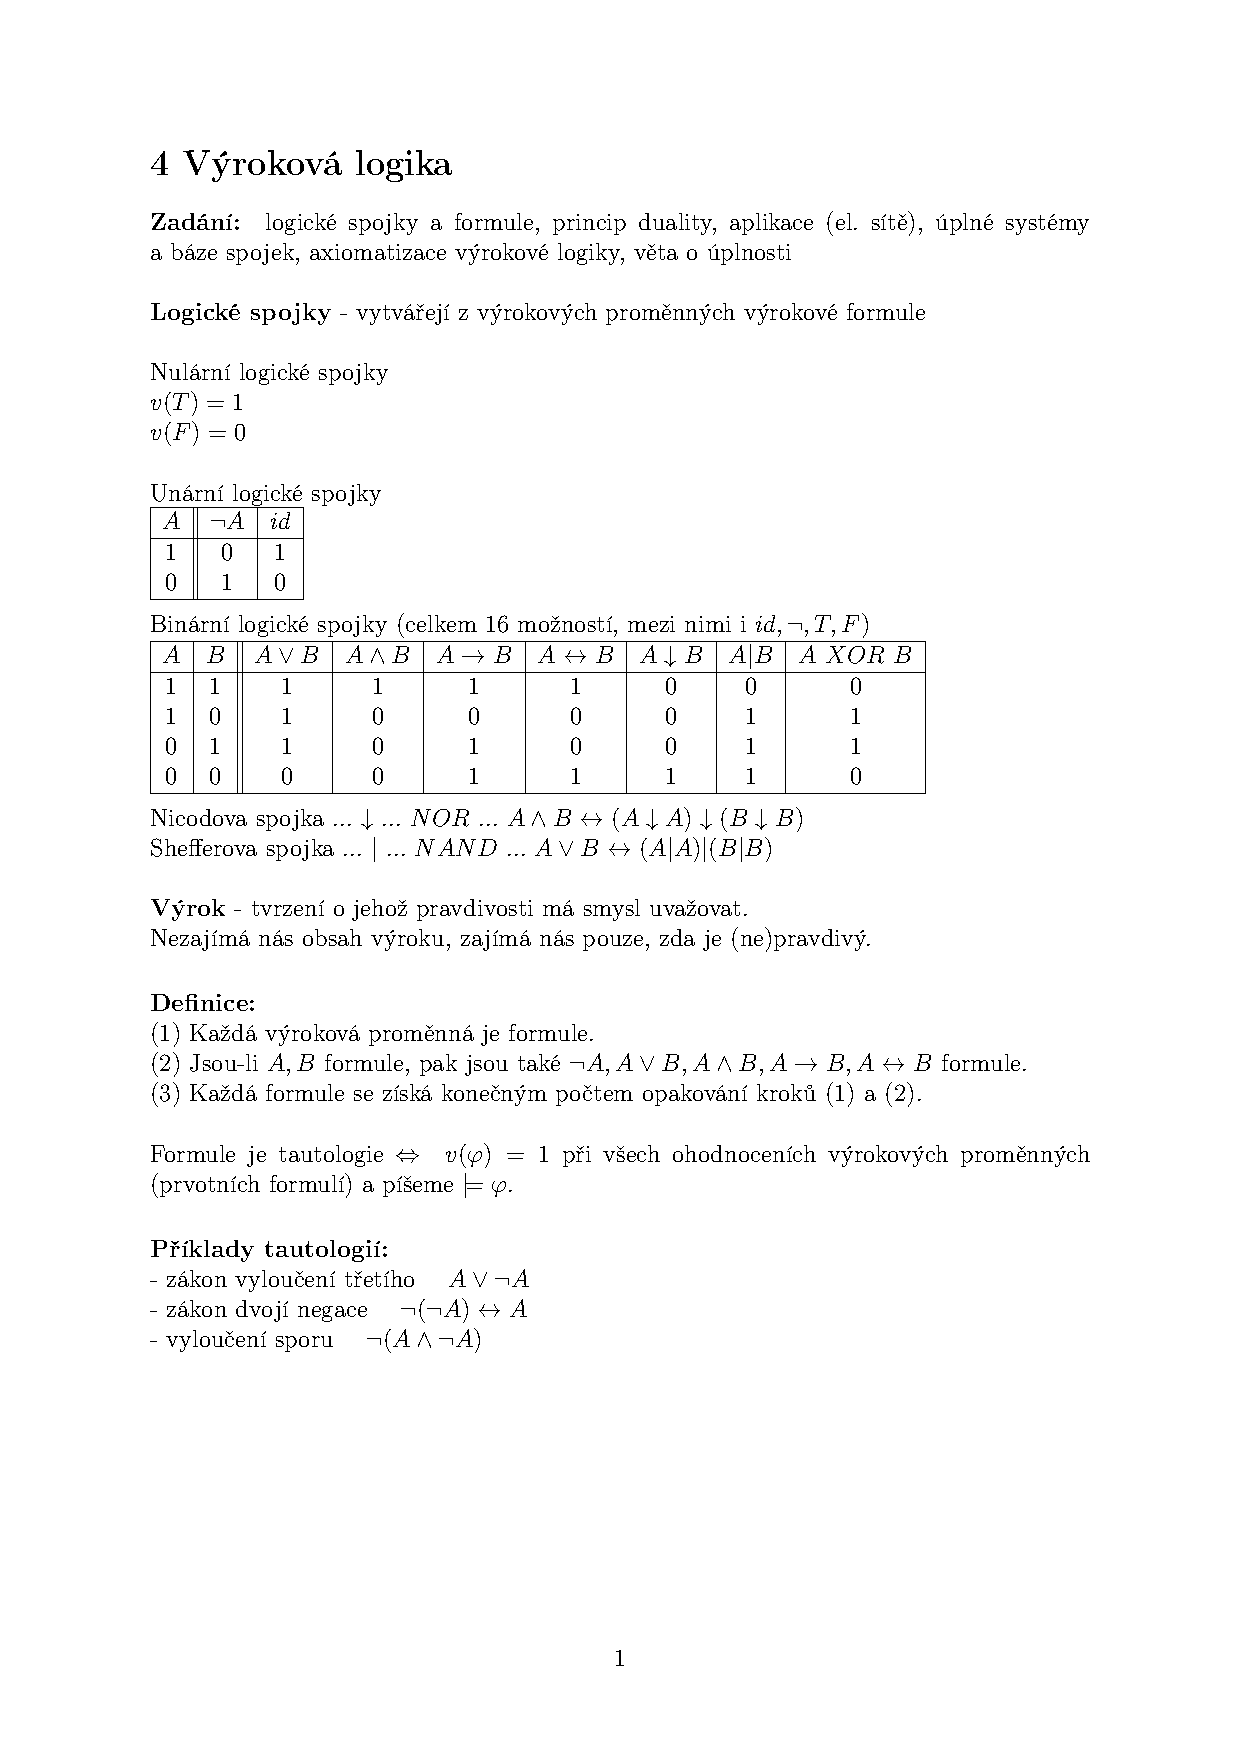
\includepdf[pages={1}]{logic_0506.pdf}
% \includepdf[pages={2}]{logic_0506.pdf}
% \includepdf[pages={3}]{logic_0506.pdf}
\paragraph*{Zadání:}
logické spojky a formule, princip duality, aplikace (el. sítě),
úplné systémy a~báze spojek, axiomatizace výrokové logiky, věta o úplnosti\\
~\\
\textbf{Logické spojky} - vytvářejí z výrokových proměnných výrokové formule\\~\\
Nulární logické spojky\\
$v(T) = 1$\\
$v(F) = 0$\\~\\
%
Unární logické spojky\\
\begin{tabular}{|c||c|c|}
\hline 
$A$ & $\neg A$ & $id$ \\ 
\hline 
1 & 0 & 1 \\ 
0 & 1 & 0 \\ 
\hline 
\end{tabular} ~\\~\\
%
Binární logické spojky (celkem 16 možností, mezi nimi i $id$ tj. identita, $\neg$, $T$ tj. tautologie, $F$ tj. negace tautologie)\\
\begin{tabular}{|c|c||c|c|c|c|c|c|c|}
\hline 
$A$ & $B$ & $A \vee B$ & $A \wedge B$ & $A \rightarrow B$ & $A \leftrightarrow B$ & $A\downarrow B$ & $A\vert B$ & $A~XOR~B$ \\ 
\hline 
1 & 1 & 1 & 1 & 1 & 1 & 0 & 0 & 0 \\ 
1 & 0 & 1 & 0 & 0 & 0 & 0 & 1 & 1 \\ 
0 & 1 & 1 & 0 & 1 & 0 & 0 & 1 & 1 \\ 
0 & 0 & 0 & 0 & 1 & 1 & 1 & 1 & 0 \\ 
\hline 
\end{tabular} ~\\~\\
Nicodova spojka ... $ \downarrow $ ... $NOR$ ... $A\wedge B \leftrightarrow (A\downarrow A)\downarrow (B\downarrow B)$\\
Shefferova spojka ... $ \vert $ ... $NAND$ ... $A\vee B \leftrightarrow (A\vert A)\vert (B\vert B)$\\~\\
%
\textbf{Výrok} - tvrzení o jehož pravdivosti má smysl uvažovat.\\
Nezajímá nás obsah výroku, zajímá nás pouze, zda je (ne)pravdivý.

\paragraph*{Definice:} ~\\
(1) Každá výroková proměnná je formule.\\
(2) Jsou-li $A, B$ formule, pak jsou také $ \neg A, A \vee B, A \wedge B, A \rightarrow B, A \leftrightarrow B $ formule.\\
(3) Každá formule se získá konečným počtem opakování kroků (1) a (2).\\
~\\
Formule je tautologie $\Leftrightarrow ~ v(\varphi ) = 1$ při všech ohodnoceních výrokových proměnných (prvotních formulí) a píšeme $\models \varphi $.
%
\paragraph*{Příklady tautologií:}~\\
- zákon vyloučení třetího ~~ $ A \vee \neg A $\\
- zákon dvojí negace ~~ $ \neg ( \neg A) \leftrightarrow A$\\
- vyloučení sporu ~~ $ \neg ( A \wedge \neg A ) $
%\newpage
\subsection*{Princip duality}
\paragraph*{Věta:}
Buď $A$ formule, v níž se vyskytují jen spojky $\neg , \vee , \wedge $.
Označme $ A ' $ formuli, která vznikne z $A$ nahrazením spojek $ \vee $, $ \wedge $
spojkami k nim duálními. Pak:\\
- $A$ tautologie $ \Leftrightarrow ~~ \neg A ' $ je tautologie\\
- je-li $(A \rightarrow B)$ tautologie, pak je také $(B' \rightarrow A')$ tautologie\\
- je-li $(A \leftrightarrow B)$ tautologie, pak je také $(A' \leftrightarrow B')$ tautologie

\paragraph*{Definice:}
Buď $A$ formule. Pak duální formulí k $A$ rozumíme $A^*$, která vznikne z $A$ záměnou spojek $ \vee , \wedge $ za spojky k nim duálními a nahrazením jednotlivých proměnných jejich negacemi.

\paragraph*{Věta:}
Buďte $A, B$ formule obsahující jen spojky $\neg , \vee , \wedge $.\\
Je-li $(A \rightarrow B)$ tautologie, pak je také $(B^* \rightarrow A^* )$ tautologie.\\
Je-li $(A \leftrightarrow B)$ tautologie, pak je také $(A^* \leftrightarrow B^* )$ tautologie.

\subsection*{Aplikace}
Spínačové obvody\\
disjunkce ... paralelní zapojení\\
konjunkce ... sériové zapojení\\
~\\
Sítě jsou ekvivalentní $\Leftrightarrow $ proud prochází oběma zároveň.\\
Minimalizace sítě\\
- minimální sít má mezi všemi sítěmi s ní ekvivalentními nejméně spínačů\\
- řešení - síť převedeme na formuli a tu upravíme na logicky ekvivalentní formuli\\
- můžeme použít Carnaughovu mapu

\paragraph*{Definice:}~\\
- \textbf{Úplným systémem spojek} výrokové logiky rozumíme takovou množinu spojek, že každou spojku výrokové logiky můžeme vyjádřit pomocí spojek z této množiny.\\
- Minimální úplný systém spojek - \textbf{báze spojek} výrokové logiky. (minimální vzhledem k množinové inkluzi)

\paragraph*{Věta:}
Jedinými bázemi spojek tvořenými jednou binární spojkou jsou $ \{ \downarrow \} $ a $ \{ \mid \} $.
%\newpage
\subsection*{Formální axiomatický systém výrokové logiky}
Abeceda\\
- množina $P$ prvotních formulí\\
- symboly pro logické spojky\\
- pomocné symboly pro závorky\\~\\
Formule\\
- všechny prvotní formule jsou formule\\
- jsou-li $A, B$ formule, pak také $\neg A, (A \rightarrow B)$ (konečná kombinace) jsou formule\\~\\
Axiomy výrokové logiky\\
(A1) $A \rightarrow (B \rightarrow A)$\\
(A2) $(A \rightarrow (B \rightarrow C)) \rightarrow (( A\rightarrow B) \rightarrow (A\rightarrow C)) $\\
(A3) $ (\neg B \rightarrow \neg A) \rightarrow (A\rightarrow B)$ ... toto je důkaz sporem\\~\\
Odvozovací pravidlo - modus ponens (pravidlo odloučení)\\
Z formulí $A, (A \rightarrow B)$ (předpoklady) se odvodí formule $B$ (závěr).

\paragraph*{Definice:}
Důkazem ve formální výrokové logice rozumíme libovolnou konečnou posloupnost $A_1 ,... A_n $ výrokových formulí takovou, že pro každé $i \leq n$ je formule $A_i$ buď axiomem nebo závěrem pravidla modus ponens.\\
$\vdash A$ ... formule $A$ je dokazatelná

\paragraph*{Věta (o dedukci):}
Nechť $T$ je množina formulí, nechť $A, B$ jsou formule.\\
Potom $T \vdash A \rightarrow B$ právě když $T \cup \{ A \} \vdash B$.

\paragraph*{Věta (o korektnosti):}
$\vdash \varphi \rightarrow \models \varphi$\\
tj. když je něco dokazatelné, tak je to tautologie

\paragraph*{Věta (o úplnosti):}
$\models \varphi \rightarrow \vdash \varphi $

\paragraph*{Lemma:} ~\\
(a) $\vdash \neg A \rightarrow (A \rightarrow B)$\\
(b) $\vdash \neg \neg A \rightarrow A$\\
(c) $\vdash A \rightarrow \neg \neg A$\\
(d) $\vdash (A\rightarrow B) \rightarrow (\neg B \rightarrow \neg A)$\\
(e) $\vdash A \rightarrow (\neg B \rightarrow \neg(A\rightarrow B)) $\\
(f) $\vdash (\neg A \rightarrow A) \rightarrow A $

\section{Predikátová logika}
% zakomentovano, protože byl vložen LaTeX kod primo... pro jistotu ponechano jako koment
% \includepdf[pages={4}]{logic_0506.pdf}
\paragraph*{Zadání:}
jazyk (termy, atomické formule a formule) a sémantika (realizace jazyka a~ohodnocení proměnných), logicky platné formule\\
~\\
Jazyk\\
- proměnné ($x$, $y$,...)\\
- speciální symboly (predikátové, funkční)\\
- výrokové spojky\\
- kvantifikátory $\forall , \exists$\\
- pomocné symboly (závorky)

\paragraph*{Term} je\\
(i) každá proměnná (i každá konstanta)\\
(ii) n-tice termů $f(t_1,t_2,...,t_n)$\\
(iii) každý term vznikne konečným počtem užití (i) a (ii)
\paragraph*{Atomická formule} ~\\
- jeden predikátový symbol $p$ aplikovaný na n-tici prvků $p(t_1,t_2,...,t_n)$
\paragraph*{Formule predikátové logiky} ~\\
(i) každá atomická formule je formule\\
(ii) jsou-li $\varphi , \psi$ formule, pak také jejich spojení pomocí spojek výrokové logiky jsou formule\\
(iii) je-li $x$ proměnná a $ \varphi $ formule, pak také $\forall x \varphi , \exists x \varphi$ jsou formule\\
(iiii) každá formule vznikne konečným počtem užití (i), (ii) a (iii)\\~\\
%
Proměnné ve formuli\\
- vázané - nachází-li se v nějaké podformuli\\
- volné - ty, které nejsou vázané\\~\\
%
Formule s čistými proměnnými\\
- otevřená formule - neobsahuje žádnou vázanou proměnnou\\
- uzavřená formule - neobsahuje žádnou volnou proměnnou

\paragraph*{Realizace $ \mathcal{R} $ jazyka} ~\\
(i) neprázdná podmnožina $M$ - univerzum\\
(ii) pro $\forall $ funkční symbol $f$ četnosti $n$ je dáno zobrazení $f_r : M^n \rightarrow M$\\
(iii)pro $\forall $ predikátový symbol $p$ četnosti $n$ ($n$-ární), kromě "$=$", je dána relace $p_r \subseteq M^n$\\~\\
%
\textbf{Ohodnocení proměnných} je libovolné zobrazení $e$ množiny všech proměnných do univerza $M$ dané realizace $\mathcal{R} $ jazyka L.\\~\\
%
Formule je \textbf{logicky platná}, jestliže pro $\forall $ realizaci $\mathcal{R} $ jazyka L je $M \models \varphi $. Píšeme $\models \varphi $.\\
Formule je pravdivá při ohodnocení $e$ v $\mathcal{R} $ ... $\mathcal{R} \models \varphi / e$\\
Formule je splněna v $\mathcal{R} $ ... $\mathcal{R} \models \varphi $

\section{Axiomatický systém predikátové logiky}
% zakomentovano, protože byl vložen LaTeX kod primo... pro jistotu ponechano jako koment
% \includepdf[pages={5}]{logic_0506.pdf}
\paragraph*{Zadání:}
axiomy a odvozovací pravidla, dokazování formulí, věta o dedukci, věty o úplnosti a bezespornosti\\~\\
%
\textbf{Axiomy výrokové logiky}\\
(A1) $A \rightarrow (B \rightarrow A)$\\
(A2) $(A \rightarrow (B \rightarrow C)) \rightarrow (( A\rightarrow B) \rightarrow (A\rightarrow C)) $\\
(A3) $ (\neg B \rightarrow \neg A) \rightarrow (A\rightarrow B)$\\~\\
%
\textbf{Axiom kvantifikátoru}\\
pokud $\varphi $ nemá volný výskyt proměnné $x$, pak $\forall x (\varphi \rightarrow \psi ) \rightarrow (\varphi \rightarrow \forall x \psi )$\\
%
\textbf{Axiom substituce}\\
pokud $t$ je term substituovatelný za $x$ do $\varphi $, pak $\forall x \varphi \rightarrow \varphi x [t]$\\
%
Je-li $L$ jazyk s rovností: \textbf{Axiom rovnosti}\\
$x_1 = y_1 \rightarrow ( ... (x_n = y_n \rightarrow (p(x_1,...,x_n)\rightarrow p(y_1,...,y_n))) ... )$\\
%
\textbf{Pravidlo odloučení} - modus ponens (MP)\\
$A, (A \rightarrow B) \vdash B$\\
%
\textbf{Pravidlo zobecnění} - modus generalis (MG)\\
$\varphi \vdash \forall x \varphi $

\paragraph*{Věta (o dedukci):}
Nechť $T$ je množina formulí, $\varphi $ je uzavřená, pak\\
$T \vdash \varphi \rightarrow \psi$ právě když $T, \varphi \vdash \psi$.\\~\\
%
Pravidlo $\forall $: Nemá-li $\varphi $ volnou proměnnou $x$: $\vdash \varphi \rightarrow \psi ~ \Rightarrow ~ \vdash \varphi \rightarrow \forall x \psi $\\
%
Pravidlo $\exists $: Nemá-li $\varphi $ volnou proměnnou $x$: $\vdash \varphi \rightarrow \psi ~ \Rightarrow ~ (\exists x \varphi ) \rightarrow \psi $

\paragraph*{Prenexní tvary formulí (dokazování formulí)} ~\\
Formule $A$ je v prenexním tvaru, jestliže má tvar $Q_1 x_1 ... Q_n x_n B$, kde\\
(i) $n \geq 0 $ a pro $\forall i=1,...,n $ je $Q_i $ buď $\forall $ nebo $\exists $\\
(ii) $x_1,...,x_n$ jsou navzájem různé proměnné\\
(iii) $B$ je otevřená formule (bez kvantifikátorů)

\paragraph*{Věta:}Ke každé formuli $A$ lze sestrojit prenexní formuli $A'$ tak, že $\vdash A \leftrightarrow A'$.% \\~\\
%Postup:\\
%bude doplněno ???

\paragraph*{Definice:} Důkaz je konečná posloupnost formulí, kde každá formule je buď axiom nebo závěr pravidla MP nebo MG.

\paragraph*{Věta o korektnosti:}
$T \vdash \varphi \Rightarrow T \models \varphi $

\paragraph*{Věta o úplnosti:}
Jestliže je $T$ teorie s jazykem $L$ a $\varphi $ je lib. formule jazyka $L$, potom $T \vdash \varphi \Leftrightarrow T \models \varphi $.\\
~\\
Teorie $T$ je bezesporná právě tehdy, když má model.



\section{Vícehodnotová logika}

\subsection{Łukasiewiczova logika}
Množinu logických hodnot budeme značit $L=\langle 0,1 \rangle$, což vyjadřuje pravdivost. Logickou proměnnou budeme nazývat takovou proměnnou, která nabývá hodnot z L. Množina logických spojek je následující:
$$S=\{\wedge, \vee,  \Rightarrow, \& \}$$
 Poslední spojka se jmenuje "odvážné a". Ve dvouhodnotové logice $\wedge$ a $\&$ splývají. Spojka \& se smí použít pouze v případě, kdy výroky, mezi které ji dáváme, jsou nezávislé co se zdroje týče (to se dá pouze předpokládat). 


\begin{definition}
\begin{itemize}
    \item Je-li $\alpha\in L \Rightarrow  \alpha $ je formule
    \item Je-li $x\textrm{ logická proměnná} \Rightarrow x$ je formule
    \item Jsou-li  $\phi$ a $\psi$ formule a $*\in S\Rightarrow (\phi * \psi )$ je logická formule
    \item Každá formule vznikla konečným použitím předešlých pravidel
\end{itemize}

\end{definition}

Dále definujeme další (pomocné) logické spojky, které umožní zjednodušit zápis.

\begin{definition}
\begin{itemize}
\item  biimplikace, oboustranná implikace: $\Leftrightarrow$ budeme psát místo $(A\Rightarrow B) \wedge (B\Rightarrow A) $
\item  Negace: $\neg$ budeme psát místo $A\Rightarrow 0$
\end{itemize}
\end{definition}

Interpretace formule nazýváme dosazení konkrétních logických hodnot do všech logických proměnných formule.

\begin{definition}
Pravdivostní ohodnocení $V(\phi)$ formule $\phi$ je zobrazení, které každé interpretaci formule $\phi$ přiřazuje logickou hodnotu z $L$.
\end{definition}


Axiomy Łukasiewiczovy logiky
\begin{itemize}
\item  $V(\alpha)=\alpha \ \ \ \forall \alpha\in L$
\item  $V(\phi \wedge \psi)=min\{ V(\phi),V(\psi)  \}$
\item  $V(\phi \vee \psi)=max\{ V(\phi),V(\psi)  \}$
\item  $V(\phi \Rightarrow \psi)=min\{1,1- V(\phi)+V(\psi)  \}$
\item  $V(\phi \& \psi)=max\{0,V(\phi)+V(\psi)-1  \}$
\end{itemize}

Klasická dvojhodnotová logika je speciálním případem výše uvedené (axiomy 2 a 5 jsou totožné).

Axiomy vícehodnotové logiky od Łukasiewicze nejsou jediné možné. Byl sestaven obecně přijímaný seznam požadavků, který by mělo splňovat pravdivostní ohodnocení. Požadavek, který je kladený na operaci, která provádí pravdivostní ohodnocení konjukce, zní, že by měla být t-normou. Požadavek kladený na disjunkci zní, že by měla být t-konormou. U implikace neexistují jednotně přijímané požadavky. Dále si uvedeme některé zobecněné implikace

\begin{itemize}
\item $I(x,y)=max\{1-x,y \}$ (Kleene-Dienes)
\item  $I(x,y)=1-x+xy$  (Rechenbach)
\item  $I(x,y)=min\{1,1-x+y\}$  (Łukasiewicz)
\item  $I(x,y)=1$ pro $x\leq y$ a $I(x,y)=y$ pro $x>y$  (Gödel)
\end{itemize}


\subsection{T-norma (trojúhelníková norma)}

\begin{definition}
Zobrazení $t:\langle 0,1\rangle \times \langle 0,1\rangle \rightarrow \langle 0,1\rangle$ se nazývá t-norma, splňuje-li následující podmínky:

\begin{itemize}
\item  t je neklesající v obou argumentech
\item  $t(x,y)=t(y,x)$  $\forall x,y\in \langle 0,1 \rangle$ (komutativita)
\item  $t(x,t(y,z))=t(t(x,y),z) $  $\forall x,y,z\in \langle 0,1 \rangle$ (asociativita)
\item $t(1,x)=x$  $\forall x\in \langle 0,1 \rangle$ (hraniční podmínka)
\end{itemize}
\end{definition}

Základní t-normy:
\begin{itemize}
\item Minimová: $T_M (x,y)=min\{x,y\}$,
\item Součinová: $T_P (x,y)=xy$,
\item Łukasiewiczova: $T_L (x,y)=max\{0,x+y-1\}$,
\item Drastický součin: $T_D(x,y)=min\{x,y\}$ pokud $max\{x,y\}=1$ jinak $T_D(x,y)=0$.
\end{itemize}



\subsection{T-konorma (trojúhelníková konorma)}

\begin{definition}
Zobrazení $s:\langle 0,1\rangle \times \langle 0,1\rangle \rightarrow \langle 0,1\rangle$ se nazývá t-konorma, splňuje-li následující podmínky:
\begin{itemize}
\item  t je neklesající v obou argumentech
\item  $s(x,y)=s(y,x)$  $\forall x,y\in \langle 0,1 \rangle$ (komutativita)
\item  $s(x,s(y,z))=s(s(x,y),z) $  $\forall x,y,z\in \langle 0,1 \rangle$ (asociativita)
\item $s(0,x)=x$  $\forall x\in \langle 0,1 \rangle$ (hraniční podmínka)
\end{itemize}
\end{definition}

Příklady t-konormy:
\begin{itemize}
\item Maximová: $S_M (x,y)=max\{x,y\}$, 
\item Pravděpodobnostní součet: $S_P(x,y)=x+y-xy$, 
\item Łukasiewiczova: $S_L (x,y)=min\{1,x+y\}$,
\item Drastický součet: $S_D(x,y)=max\{x,y\}$ pokud $min\{x,y\}=0$ jinak $S_D(x,y)=1$.
\end{itemize}







\section{NP úplné úlohy}

\section{Slovní modely}

\begin{definition}
Formule
\end{definition}

\begin{definition}
Nechť $X_1,...,X_n$ jsou slovní proměnné, $\Theta(t_1,...,t_n)$ je formule, $L_1,...,L_n$ slovní hodnoty $X_1,...,X_n$. $\mu_{L_1}(y_1),...,\mu_{L_n}(y_n)$ jsou sémantické interpretace těchto slovních hodnot. Položme $t_1=\mu_{L_1}(y_1),...,t_n=\mu_{L_n}(y_n)$, pak $\Theta(t_1,...,t_n)$ je \textbf{slovním modelem}. 
\end{definition}

\begin{definition}
$X_1,...,X_n$ jsou nezávislé slovní proměnné a $L_1,...,L_n$ jejich slovní hodnoty. Nechť $y$ je závislá slovní proměnná a $K$ její slovní hodnota.\textbf{CI-prohlášením} nazveme slovní model když $$x_1=L_1,...,x_n=L_n \quad \Longrightarrow \quad y=K$$
\end{definition}

\begin{definition}
Nechť $P_1,...,P_n$ jsou CI prohlášení, pak $P_1\wedge P_2\wedge...\wedge P_n$ nazveme \textbf{CIC} modelem a $P_1 \& P_2 \&... \& P_n$ \textbf{CI\& modelem}.
\end{definition}

\begin{definition}
Nechť $X_1,...,X_n$ jsou slovní proměnné, které definujeme, že jsou známé a slovní proměnnou $Y$, kterou definujeme, že je neznámá. $L_1,...,L_n$ nechť jsou slovní hodnoty známých proměnných. $K$ slovní hodnota neznámé proměnné. $$x_1=L_1\wedge...\wedge x_n=L_n \quad \wedge \quad Y=K$$ nazveme \textbf{CC prohlášením}
\end{definition}

\begin{definition}
Nechť $Q_1,...,Q_n$ jsou CC prohlášení. Pak $Q_1 \vee...\vee Q_n$ nazveme \textbf{CCD modelem}.
\end{definition}

Shrnutí vlastností slovních modelů:
\begin{center}
 \begin{tabular}{|| c ||c c c c||} 
 \hline
  & interpretace pravdy & citlivost na spory & citlivost na redund. info. & přezdívka \\ [0.5ex] 
 \hline\hline
 CCD & pravda je to, co tvrdí alespoň jedno prohlášení & ne & ne & naivní hazardér \\ 
 \hline
 CIC & pravda je to, co není v rozporu s libovolným prohlášením & ano & ne & zbabělý inteligent \\
 \hline
 CI\& & pravda je to, co není v rozporu s libovolným prohlášením & ano & ano & Göbbels \\ [1ex] 
 \hline
 \end{tabular}
\end{center}

\section{Matematické struktury}
